\section{Place \& Route}
\begin{figure}
		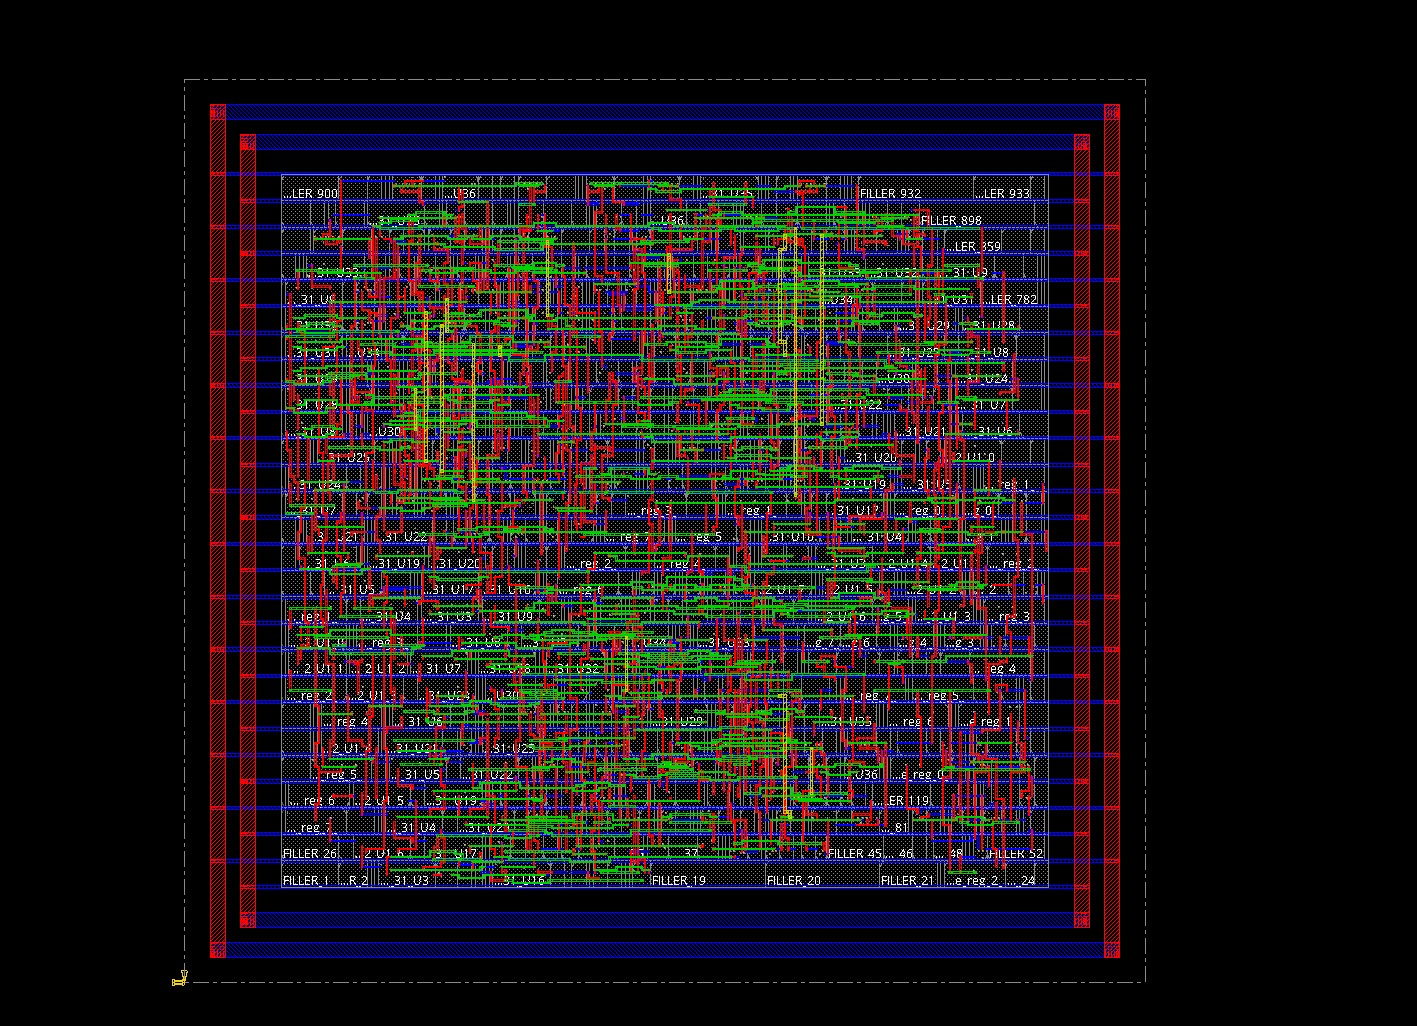
\includegraphics[width=\textwidth]{./chapter5/pic.jpg}
		\caption{Snapshot after routing}
\end{figure}
\paragraph{Global routing} This step ends without reporting any critical error, the final summary shows the overall routed length for each metal layer involved:\todo{Copy and paste log file}


\paragraph{Timing analysis} The worst slack is $8.56\,\textrm{ns}$, slighly larger than the one found in Synopsys ($8\,\textrm{ns}$). The same situation occurs with the look-ahead architecture.


\paragraph{Connectivity verification} The are 0 warning or violations for this step.


\paragraph{Gate count} Total area and cell/gate count is:
\begin{center}
    \begin{tabular}{|l|l|}
	   \hline
	   Gates & 1143 \\
	   Cells &     459 \\
	   Area &     912.4 um$^2$\\\hline
    \end{tabular}
\end{center}


\paragraph{Power analysis} Results are reported in \autoref{tab:post_pr_power_report}. The total power is slightly larger than the one computed by Synopsys (\autoref{tab:power_report_standard}), this could be expected since Innovus takes into account resistive and capacitive parasitics that will only increase power dissipation.

\begin{table}
	\centering
\begin{tabular}{|l|l|l|l|l|}
	\hline
\textbf{Group}                &           \textbf{Internal  Power} &  \textbf{Switching  Power}  &   \textbf{Leakage  Power}     & \textbf{Total  Power} \\
\hline
Sequential       &                  0.03623  &  0.001813  &  0.004147   &  0.04219 (18.21\%)  \\
Macro                       &           0    &       0       &    0      &     0  \\
IO                         &            0       &    0     &      0      &     0 \\
Combinational                &     0.09489  &   0.07816  &   0.01643   &   0.1895 (81.79\%)  \\
Clock (Combinational)        &          0      &     0     &      0    &       0  \\
Clock (Sequential)             &        0     &      0      &     0     &      0 \\
\hline
Total                      &      0.1311  &   0.07997  &   0.02057   &   0.2317 (100\%) \\\hline
\hline
\textbf{CLK}                         &    0.03587 &   0.001562  &  0.003817  &   0.04125 (17.81\%) \\\hline
\end{tabular}
\caption{Power report after place \& route: Group Power for Rail VDD and CLK}
\label{tab:post_pr_power_report}
\end{table}
